%\documentclass[a4paper,english,12pt,twocolumn]{article}
\documentclass[a4paper,english,11pt]{article}
\usepackage[utf8]{inputenc} % Encodage du fichier
\usepackage[T1]{fontenc} % Encodage des fonts nécessaire pour le Latin
\usepackage[french]{babel} % Pour changer la langue des mots générés et choisir la bonne mise en page
\usepackage{amssymb}
\usepackage{pdflscape}
\usepackage{microtype} 
\usepackage{lmodern} % Le latin modèrne
\usepackage[top=2cm, bottom=2cm, left=2cm, right=2cm]{geometry} % Définir les marges de la page 
\usepackage[hidelinks,urlcolor=blue,unicode=true,
pdftitle={Détection des effets indésirables d'un médicament à partir d'un texte},
pdfauthor={BELOUADAH Eden and BOUHAHA Mariem},
pdfdisplaydoctitle=true]{hyperref} % Pour les liens 
\usepackage{fancyhdr} % Pour le style de la page
\usepackage[font=it]{caption} % Rendre les titres des tableaux italiques
\usepackage{graphicx} % Pour les images
\usepackage{subcaption} % Pour mettre plusieurs images sur la même ligne
\usepackage{float} % Pour empêcher le déplacement des tableaux et des figures.
\usepackage{babelbib} % Pour changer la langue dans la bibliographie
\usepackage{amsmath} % Pour des fonctions mathématiques
\usepackage{amssymb} % Pour les symboles mathématiques
%\usepackage[onelanguage,english,longend,boxruled,algoruled,linesnumbered,algochapter,nofillcomment]{algorithm2e} %pour les algorithmes
\usepackage{multirow}
\usepackage{booktabs}
\usepackage{enumitem}
\usepackage{setspace}
\usepackage[normalem]{ulem}
\usepackage{cancel}

\graphicspath{ {images/} } % Spécifier le répertoire contenant les images

\DisableLigatures[f]{encoding=*}

%Active ça si tu ne veux pas les points-virgules dans les algorithmes
% \DontPrintSemicolon
 
%\renewcommand \thechapter{\Roman{chapter}} % Utiliser les numéros romans pour les chapitres

\captionsetup{labelfont=it,textfont=it,labelsep=period} % Changer le style des légendes
\AtBeginDocument{ % Changer les légendes
	\renewcommand\tablename{\itshape Tableau}
	\renewcommand{\figurename}{\itshape Figure}
	% Renommer la table des matières
	\renewcommand{\contentsname}{Sommaire}
}

% Style de l'entête et le pied de la page
\setlength{\headheight}{16pt}
\pagestyle{fancy}
\fancyhead[L]{} % Enlever la section
\fancyhead[R]{\footnotesize\slshape{\nouppercase{\leftmark}}} % Titre du chapitre en minuscule avec taille 10
\fancyfoot[C]{}
\fancyfoot[R]{\thepage} % Déplacer le numéro de la page vers la droite de la page

\fancypagestyle{plain}{
\renewcommand{\headrulewidth}{0pt}
\fancyhf{}
\fancyfoot[R]{\thepage}
}
  
% Espace entre les lignes
\linespread{1.3}

% Code pris de https://tex.stackexchange.com/a/95616/109916 et corrigé
% Début
\makeatletter
\newcommand{\emptypage}[1]{
  \cleardoublepage
  \begingroup
  \let\ps@plain\ps@empty
  \pagestyle{empty}
  #1
  \cleardoublepage
  \endgroup}
\makeatletter
% Fin


% pour changer les deux points des légendes d'algorithmes
% \SetAlgoCaptionSeparator{\unskip.}

\begin{document}
%\include{Page_de_garde}
%\include{Remerciements}
\emptypage{
%\tableofcontents
%\listoffigures
%\listoftables
}
    
\setlength{\parskip}{0.6em plus 0.1em minus 0.1em}
%\SetKwInput{KwOut}{Outpits}

% Redéfinition des chapitres et sections pour les inclure dans le sommaire
\makeatletter
%	\let\oldchapter\chapter
%	\newcommand{\@chapterstar}[1]{\cleardoublepage\phantomsection\addcontentsline{toc}{chapter}{#1}{\oldchapter*{#1}}\markboth{#1}{}}
%	\newcommand{\@chapternostar}[1]{{\oldchapter{#1}}}
%	\renewcommand{\chapter}{\@ifstar{\@chapterstar}{\@chapternostar}}
\let\oldsection\section
\newcommand{\@sectionstar}[1]{\phantomsection\addcontentsline{toc}{section}{#1}{\oldsection*{#1}}}
\newcommand{\@sectionnostar}[1]{{\oldsection{#1}}}
\renewcommand\section{\@ifstar{\@sectionstar}{\@sectionnostar}}	
\newcommand*{\rom}[1]{\expandafter\@slowromancap\romannumeral #1@}
\makeatother

\setcounter{page}{1}
%%%%%%%%%%%%%%%%%%%%%%%%%%%%%%%%%%%%%%%%%%%%%%%%%%%%%%%%%%%%%

\title{Détection des effets indésirables d'un médicament à partir d'un texte}
\author{Eden Belouadah \and Bouhaha Mariem}
% \date{}
\maketitle

\section{Introduction}
L'intelligence artificielle a connu de nombreuses applications sur le domaine médical. En effet, nous trouvons souvent des méthodes qui servent à faciliter la vie des patients et à aider les médecins à bien gérer et comprendre les causes des maladies de leur patients en plus d'avoir des statistiques et comprendre des informations difficiles à détecter par l'être humain sur la grande échelle.

Ce projet consiste à développer un système automatique de détection des effets indésirables d'un médicament à partir d'une notice ou d'un texte quelconque. Nous utilisons pour cette tâche le Thésaurus MedDRA [1].

L'hypothèse de base est de tester Wapiti CRF [2] sur un fichier de base qui contient le mot et sa classe séparés par une tabulation.

\section{Matériel}
Les données mises à notre disposition pour cette tâche sont les suivantes:

\begin{itemize}
	\item Un corpus de format \emph{brat}, qui permet de visualiser les concepts d'effets secondaires pour bien comprendre la tâche et s'inspirer pour trouver des idées innovantes. Exemple:
	
	\begin{figure}[H]
		\centering
		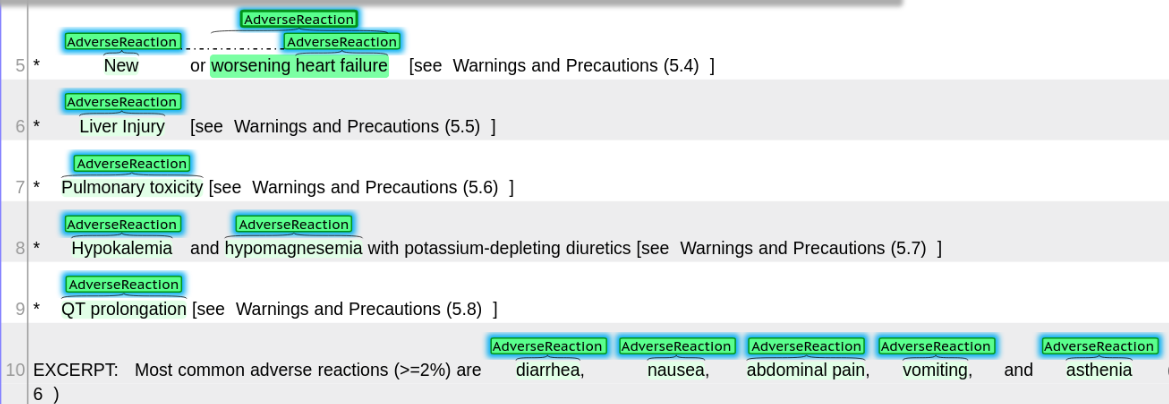
\includegraphics[width=0.8\textwidth,keepaspectratio]{fichier_brat}
		\caption{Fichier de format brat pour la notice du médicament AMPYRA\label{}}
	\end{figure}
		
	\item Un corpus qui contient 101 fichiers. Chaque fichier (de format tabulaire) correspond à une notice d'un médicament. Par exemple:
	
	\begin{figure}[H]
		\centering
		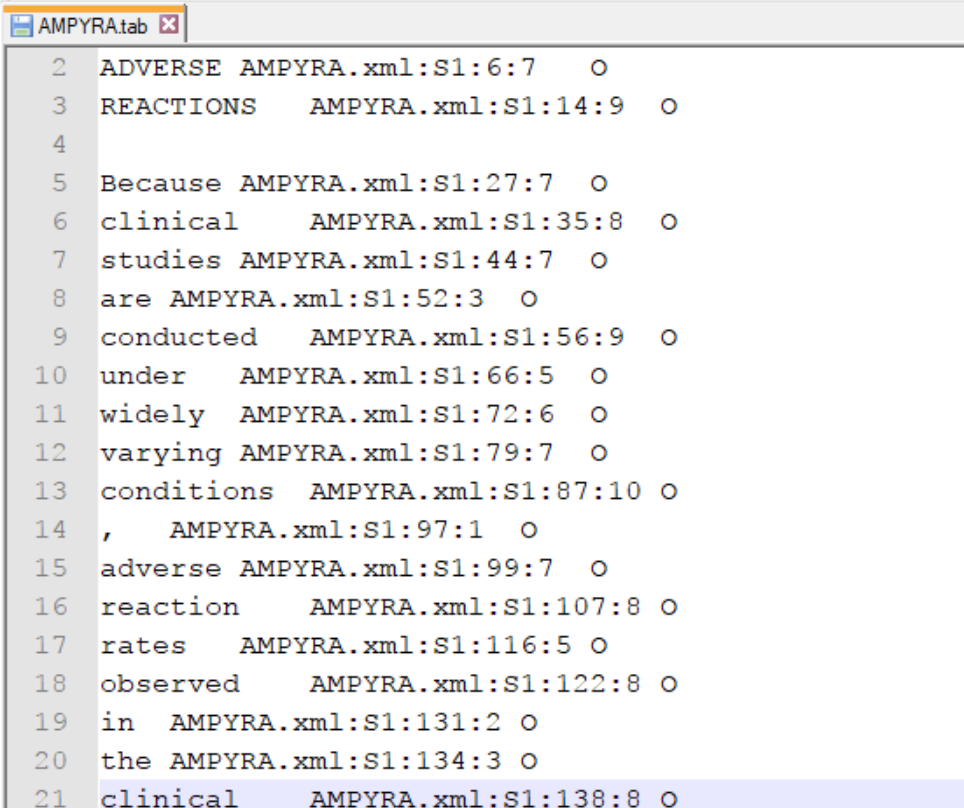
\includegraphics[width=0.6\textwidth,keepaspectratio]{fichier_tab}
		\caption{Fichier tabulaire pour la notice du médicament AMPYRA\label{}}
	\end{figure}

La première colonne correspond au mot, la deuxième correspond à la position du mot dans le fichier d'origine d'où est construit le fichier tabulaire (Cette colonne est gardée mais elle sera ignorée pendant toutes les phases de traitement). La troisième représente la classe du mot, c'est à dire, est ce que c'est un effet indésirable ou non.

Pas seulement les effets indésirables sont annotés dans les fichiers tabulaires mais tous les autres entités possibles sont annotées. L'étiquette "O" signifie que ce mot ne correspond à aucun concept, l'étiquette précédée par "B" signifie le début d'un concept et l'étiquette précédée par "I" signifie que nous somme à l'intérieur d'un concept. 

Nous nous intéressons donc aux deux étiquettes: B-AdverseReaction et I-AdverseReaction.
	
\end{itemize}

\section{Méthodes et protocole expérimental}
Avant d'entamer la partie traitement, nous avons divisé les fichiers du corpus en trois: Entrainement (60\%), développement (20\%) et test (20\%). Nous faisons l'apprentissage sur l'ensemble d'entrainement, les expérimentations et le réglage des paramètres sur l'ensemble de développement et nous gardons l'ensemble de test pour le calcul des performances finales.

\begin{table}[H]\centering
	\begin{tabular}{ccccccc}
		\toprule \textbf{Ensemble} & Entrainement & Développement & Test \\    \midrule
		\textbf{Nombre de lignes} & 152274 & 73228 & 52908  \\   
		\bottomrule	
	\end{tabular}
	\caption{Distribution des lignes dans les trois ensemble de données\label{}}
\end{table}

\subsection{Méthodes employées}
Les méthodes utilisées sont présentées sous forme d'étapes. Les performances seront représentées dans la section suivante.
\subsubsection{Etape 0: Hypothèse de base}
La méthode de base est de considérer un fichier de la forme suivante:
$$
mot\qquad \text{\cancel{nom\_fichier}}\qquad	classe		
$$
Le fichier de patrons utilisé consiste à prendre en considération le mot courant, les deux mot précédents et les deux mot suivants.

Les résultats obtenus avec ce fichier de patrons de base ne sont pas mal. Cependant, d'autres améliorations peuvent être faites.

\subsubsection{Etape 1: Bigrammes de classes}
Nous gardons la même structure de fichier d'entrée et nous modifions le fichier de patrons pour prendre en considération la classe courante, le bigramme (classe précédente, classe courante) et le bigramme (classe courante, classe suivante).

\subsubsection{Etape 2: Racinisation}
Nous ajoutons au fichier d'entrée la racine pour chaque mot. La racine permet de trouver la corrélation entre les exemples qui ont des mots qui partagent la même racine.

$$
mot\qquad \text{\cancel{nom\_fichier}}\qquad racine \qquad	classe		
$$

Nous avons testé trois racinisateurs: \emph{PorterStemmer}, \emph{LancasterStemmer} et \emph{SnowballStemmer}. Le meilleur résultat est obtenu avec \emph{PorterStemmer} donc nous l'avons gardé pour les prochaines étapes.

\subsubsection{Etape 3: Etiquetage morpho-syntaxique}
Nous nous sommes débrouillées avec l'étiqueteur de \emph{NLTK} pour ajouter les étiquettes morpho-syntaxiques correspondantes aux mots. Le fichier d'entrée a maintenant cette forme:

$$
mot\qquad \text{\cancel{nom\_fichier}}\qquad racine \qquad étiquette\qquad	classe		
$$
L'étiquetage morpho-syntaxique permet de bien  déterminer le rôle du mot dans la phrase, et faire la différence entre les catégories grammaticales de manière à bien classer le mot.

\subsubsection{Etape 4: Ne pas tenir compte de la casse}
Dans cette étape, nous n'avons pas travaillé sur la structure du fichier d'entrée mais nous avons modifié les patrons de telle manière à ne pas respecter la casse. Cette étape semble illogique vu que certains effets indésirables peuvent effectivement commencer par des majuscules, mais ça a amélioré (un peu) les résultats.

\subsubsection{\cancel{Etape 5: Lemmatisation}}
Dans cette étape, nous avons utilisé le \emph{WordNetLemmatiser} pour ajouter les lemmes des mots traités. Ce lemmatiseur nécessite l'information sur la catégorie grammaticale du mot pour pouvoir mieux fonctionner. C'est pour cette raison que nous avons d'abord commencé par ajouter les étiquettes morpho-syntaxiques.

$$
mot\qquad \text{\cancel{nom\_fichier}}\qquad racine \qquad étiquette\qquad lemme\qquad	classe		
$$

La lemmatisation n'a pas amélioré les résultats, donc nous l'avons enlevé du fichier d'entrainement.

\subsubsection{\cancel{Etape 6: Représentation vectorielle}}
Le modèle \emph{word2vec} de la bibliothèque \emph{gensim} est utilisé pour ajouter des embeddings représentant les mots comme d'autres attributs dans le fichier d'entrée. La taille des embeddings est fixée à 5. embedding=[$X_1, X_2, X_3, X_4, X_5$].
La représentation vectorielle permet de donner une représentation similaire pour les mots proches entre eux.

$$
mot\quad \text{\cancel{nom\_fichier}}\quad racine \quad étiquette\quad X_1\quad X_2\quad X_3\quad X_4\quad X_5\quad	classe		
$$

La représentation vectorielle a été appris à partir du corpus d'entrainement lui même et malheureusement n'a pas amélioré les résultats.


\subsubsection{Etape 7: Elimination des classes inutiles}
Dans cette étape, nous éliminons toutes les classes qui ne nous intéressent pas (par exemple I-Drug et B-Drug). Et cela pour alléger le travail du modèle et accélérer le temps d'apprentissage. Donc les seules classes gardées sont: B-AdverseReaction, I-AdverseReaction et O.

\subsubsection{\cancel{Etape 8: Elimination des mots vides}}
Cette étape consiste à éliminer les mots vides du corpus. Nous avons testé deux méthodes: Appel à la liste $stopwords$ de $NLTK$ et élimination des mots selon leur catégorie grammaticale (éliminer les ponctuations et les conjonctions par exemple). Cette étape n'a pas amélioré les résultats non plus.

\subsection{Protocole expérimental}
Afin de comparer les méthodes et voir si une méthode est de bonne qualité, nous regardons d'abord les critères \emph{token error} et \emph{sequence error}, puis nous mettons l'accent sur la F-mesure des deux classes \emph{B-AdverseReaction} et \emph{I-AdverseReaction}.

\section{Résultats}
Les performances obtenues sur l'ensemble de développement sont les suivantes:

\begin{table}[H]\centering
	\begin{tabular}{cccccccccc}
		\toprule \textbf{Etape} & 0 & 1 & 2 & 3 & 4 & 5 & 6 & 7 & 8\\    \midrule
		\textbf{Tokens error} & 5.59\% & 5.53\%  & 5.18\% & 4.94\% & 4.80\% & 4.89\%  & 5.36\% & \textbf{3.84\%} & 4.96\%  \\
		\textbf{Sequences error} & 35.59\% & 30.09\% & 29.58\% & 27.33\% & 26.62\% & 26.90\%  & 27.07\% & \textbf{23.71\%} & 23.62\%  \\ 
		\textbf{F(B-AdvReaction)} & 72\% & 73\% & 74\% & 75\% & 77\% & 77\%  & 72\% & \textbf{77\%} & 75\%   \\
		\textbf{F(I-AdvReaction)} &   62\% & 66\% & 68\% & 68\% &  69\% & 69\%  & 61\% & \textbf{68\%} & 67\%  \\
		\bottomrule	
	\end{tabular}
	\caption{Résultats obtenus pour les différentes étapes\label{}}
\end{table}

Les étapes hachurées sont les étapes que nous n'avons pas pris en considération dans le modèle final. Les résultats finaux sont les suivants:

\begin{table}[H]\centering
	\begin{tabular}{ccc}
		\toprule \textbf{Ensemble} & Développement & \textbf{Test}\\    \midrule
		\textbf{Tokens error} & 3.84\% & \textbf{3.25\%}  \\
		\textbf{Sequences error} & 23.71\% & \textbf{16.71\%} \\
		\textbf{F$_{mesure}$(B-AdverseReaction)} & 77\% & \textbf{86\%}\\
		\textbf{F$_{mesure}$(I-AdverseReaction)} &   68\% & \textbf{74\%} \\
		\bottomrule	
	\end{tabular}
	\caption{Résultats finaux pour le développement et le test}
\end{table}



\section{Discussion des résultats}
Nous remarquons que les résultats s'améliorent d'une étapes à une autre, sauf pour certaines étapes que nous avons décidé de ne pas prendre en considération. Les résultats sont l'ensemble de Test sont très bons par rapports aux résultats que nous avons obtenu lors de la phase de développement.

Il n'y a pas une étape qui a permis de faire un grand saut dans les résultats, mais chaque étape a contribué d'un petit pourcentage dans l'amélioration des résultats. La présentation des résultats détaillés permet de voir l'importance de chaque chaque étape dans le processus d'apprentissage.

\subsection{Et si on s'intéresse que si l'étiquette est AdverseReaction ou non?}
Une petite expérience simplificatrice a été faite qui sert à déterminer si un mot est un effet indésirable ou non. C'est à dire, nous avons considéré que les deux étiquettes B-AdverseReaction et I-AdverseReaction sont la même étiquette AdverseReaction. Les résultats obtenus sont les suivants:


\begin{table}[H]\centering
	\begin{tabular}{ccc}
		\toprule \textbf{Ensemble} & Développement & \textbf{Test}\\    \midrule
		\textbf{Tokens error} & 3.72\% & \textbf{3.11\%}  \\
		\textbf{Sequences error} & 23.18\% & \textbf{16.50\%} \\
		\textbf{F$_{mesure}$(AdverseReaction)} & 76\% & \textbf{82\%}\\
		\bottomrule	
	\end{tabular}
	\caption{Résultats de l'expérience simplificatrice}
\end{table}

Nous remarquons que l'hypothèse simplificatrice n'a pas beaucoup affecté les résultats du modèle.
\section{Conclusion}
L'hypothèse de base a donnée un résultat acceptable mais il fallait l'enrichir encore pour améliorer les résultats. Parmi les perspectives envisageables, on peut penser à se servir d'autres ressources externes qui permettent de bien caractériser les mots. Ces ressources peuvent être médicales aussi bien que linguistiques.

Ce projet représente un exemple de nombreuses applications de l'apprentissage automatique qui sont dédiées au domaine médical. La détection des effets indésirables peut être étendue à d'autres tâches similaires telles la détection des traitements et des symptômes. Le domaine médical reste un domaine très vaste et plein de défis pour les informaticiens intéressées  par l'amélioration de la vie quotidienne des patients et des médecins.

\section*{Références}
[1] Thésaurus MedDRA. https://www.meddra.org/glossary

[2] Wapiti - A simple and fast discriminative sequence labelling toolkit, https://wapiti.limsi.fr.
%%%%%%%%%%%%%%%%%%%%%%%%%%%%%%%%%%%%%%%%%%%%%%%%%%%%%%%%%%%%%
\bibliographystyle{babplain}
\parskip=-1em
%\emptypage{\bibliography{bibliographie}}
\let\section\oldsection % pour éviter que le résumé soient visibles dans le sommaire comme une section
%\include{Resume}
\end{document}
